\subsection{参照値整形とレート制限}

入力飽和とアンチワインドアップを入れると、制御器の内部状態はアクチュエータの限界と矛盾しにくくなる。しかし、それだけでは目標値そのものが物理的に実行可能になるわけではない。DC モータの位置サーボで、軸角度を今すぐ $1\,\mathrm{rad}$ だけ動かすステップ目標値を与えた場合を考える。積分器が暴走しなくても、ステップ目標値は瞬間的な位置変化を要求するので、有限の電圧、電流、トルクしか出せないモータには追従できない。

簡単な検証対象として、角度を $\theta(t)\,[\mathrm{rad}]$、角速度を $\omega(t)\,[\mathrm{rad/s}]$、モータへ印加される電圧を $u(t)\,[\mathrm{V}]$ とし、動作点近傍で
\begin{align}
  \dot{\theta}&=\omega,\\
  J\dot{\omega}&=K_tu-b\omega,
  \qquad |u|\leq u_{max}
  \label{eq:reference-shaping-motor-model}
\end{align}
と近似する。ここで $J\,[\mathrm{kg\,m^2}]$ は慣性、$b\,[\mathrm{N\,m\,s/rad}]$ は粘性係数、$K_t\,[\mathrm{N\,m/V}]$ は電圧からトルクへの比例係数、$u_{max}\,[\mathrm{V}]$ は電圧上限である。位置制御器は、目標値経路から作った実際の参照値を $r_a(t)\,[\mathrm{rad}]$ として
\begin{align}
  u_c&=K_p(r_a-\theta)-K_d\omega,\\
  u&=\operatorname{sat}_{[-u_{max},u_{max}]}(u_c)
  \label{eq:reference-shaping-position-servo}
\end{align}
とする。$K_p$ の単位は $\mathrm{V/rad}$、$K_d$ の単位は $\mathrm{V/(rad/s)}$ である。微分は測定速度側に置き、目標値ステップによる微分キックは避けている。積分項を加える場合でも、アンチワインドアップは $u_c$ と $u$ の差を内部状態へ戻す処理であり、式 \eqref{eq:reference-shaping-position-servo} が飽和を受ける事実は残る。

生のステップ目標値は
\begin{equation}
  r_{step}(t)=r_0+\Delta r\,H(t-t_0)
\end{equation}
で表せる。$H$ は単位ステップであり、形式的な速度は
\begin{equation}
  \dot{r}_{step}(t)=\Delta r\,\delta(t-t_0)
\end{equation}
になる。これは、目標角度の速度が瞬間だけ無限大になることを意味する。モータ側では $|\dot{\omega}(0)|\leq K_tu_{max}/J$ なので、この要求は最初から実現できない。さらに、初期状態が $\theta=r_0,\omega=0$ なら、式 \eqref{eq:reference-shaping-position-servo} の直後の指令は
\begin{equation}
  u_c(t_0^+)=K_p\Delta r
\end{equation}
である。$|K_p\Delta r|>u_{max}$ なら、最初の計算から飽和が確定する。

この問題を、制御器ゲインだけで直すと、応答全体を遅くすることになりやすい。別の考え方は、外から来た目標値 $r_{cmd}$ をそのまま制御器へ入れず、モータが追従しやすい参照値 $r_a$ へ変換してから入れることである。この変換を参照値整形という。最も単純な整形は、時定数 $\tau_r\,[\mathrm{s}]$ の一次遅れ
\begin{equation}
  \tau_r\dot{r}_f=r_{cmd}-r_f,
  \qquad r_a=r_f
  \label{eq:first-order-reference-shaping}
\end{equation}
である。$r_{cmd}$ と $r_f$ の単位は同じ $\mathrm{rad}$ で、$\dot{r}_f$ の単位は $\mathrm{rad/s}$ である。$t=t_0$ で $r_0$ から $r_0+\Delta r$ へ変わるステップに対し、$t\geq t_0$ では
\begin{align}
  r_f(t)&=r_0+\Delta r\{1-\exp(-(t-t_0)/\tau_r)\},\\
  \dot{r}_f(t)&=\frac{\Delta r}{\tau_r}
  \exp(-(t-t_0)/\tau_r)
  \label{eq:first-order-reference-step}
\end{align}
となる。したがって初期の最大参照速度は $|\Delta r|/\tau_r$ である。$\tau_r$ を大きくすると速度要求は下がるが、目標値へ近づく時間は長くなる。

もう一つのよく使う実装は、サンプリング周期 $T_s\,[\mathrm{s}]$ ごとに変化量を制限するレートリミッタである。最大速度を $v_{max}\,[\mathrm{rad/s}]$ として
\begin{equation}
  r_{\ell,k+1}
  =
  r_{\ell,k}
  +
  \operatorname{clip}
  \left(
    r_{cmd,k}-r_{\ell,k},
    -v_{max}T_s,
    v_{max}T_s
  \right),
  \qquad r_a=r_\ell
  \label{eq:rate-limited-reference}
\end{equation}
と更新する。ここで $\operatorname{clip}(x,a,b)$ は $x$ を区間 $[a,b]$ に収める演算である。ステップ目標値に対しては、符号を除けば傾き $v_{max}$ のランプになり、移動時間は少なくとも $|\Delta r|/v_{max}$ になる。一次整形は指数関数的に滑らかに目標へ近づき、レート制限は最大速度を明示的に守る、という違いがある。

参照値がアクチュエータ制約と矛盾しているかどうかは、飽和後の入力だけを見ると分かりにくい。飽和後の $u$ は必ず範囲内に収まるからである。そこで、飽和前の指令余裕
\begin{equation}
  \mu_c(t)=1-\frac{|u_c(t)|}{u_{max}}
  \label{eq:command-margin-reference-shaping}
\end{equation}
を使う。$\mu_c(t)>0$ なら指令は電圧範囲内にあり、$\mu_c(t)=0$ はちょうど上限、$\mu_c(t)<0$ は制御器が実現できない電圧を要求している状態である。

\wfig{reference-shaping-rate-limit-examples} は、式 \eqref{eq:reference-shaping-motor-model} と式 \eqref{eq:reference-shaping-position-servo} を
\begin{equation}
  J=1.0,\quad b=0.55,\quad K_t=1.0,\quad
  u_{max}=2.2,\quad K_p=10.0,\quad K_d=3.2
\end{equation}
で計算した例である。目標値は $t_0=0.30\,\mathrm{s}$ で $\Delta r=1.0\,\mathrm{rad}$ だけ変わる。生ステップでは $u_c(t_0^+)=10.0\,\mathrm{V}$ となり、上限 $2.2\,\mathrm{V}$ の約 $4.5$ 倍を要求するため、指令余裕は大きく負になる。一次整形で $\tau_r=0.60\,\mathrm{s}$ とすると、最大参照速度は $1.67\,\mathrm{rad/s}$ になり、最小余裕はほぼ $0$ の近くまで改善する。レート制限で $v_{max}=0.90\,\mathrm{rad/s}$ とすると、余裕をさらに残したまま応答する。

\begin{figure}[tbp]
\centering
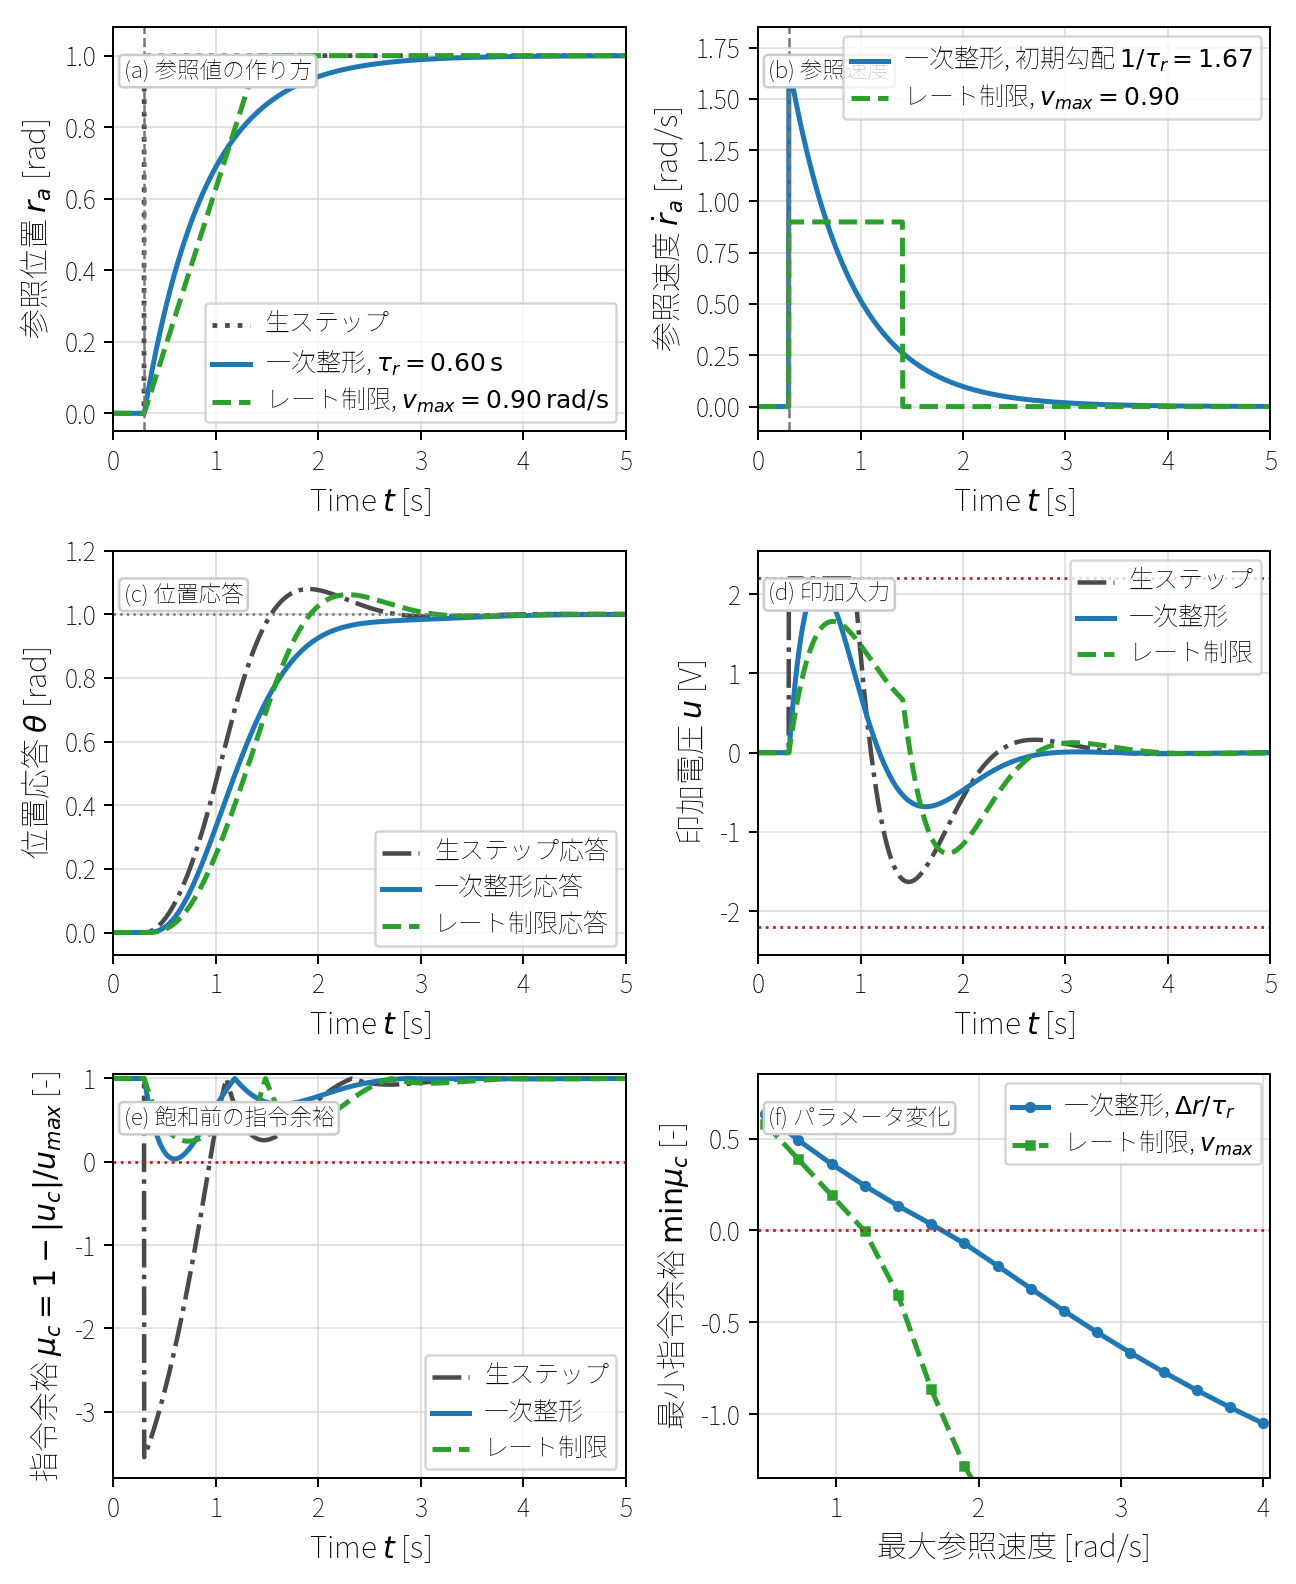
\includegraphics[width=0.96\linewidth,bb=0 0 1296 1584]{figures/reference_shaping_rate_limit_examples.png}
\caption{DC モータ位置サーボに対する参照値整形とレート制限の比較。生ステップは位置目標を瞬時に変えるため、飽和前の電圧指令が上限を大きく越える。一次整形は時定数 $\tau_r$ で参照速度を有限にし、レート制限は $v_{max}$ で参照速度そのものを制限する。下段右は最大参照速度を変えたときの最小指令余裕であり、速い参照ほど余裕が減ることを表している。}
\label{fig:reference-shaping-rate-limit-examples}
\end{figure}

パラメータの役割は、応答の見た目ではなく、制約余裕と移動時間の両方で解釈する。一次整形では、$\tau_r$ を小さくすると $|\Delta r|/\tau_r$ が大きくなり、参照値は速く立ち上がるが、図の下段右のように $\min\mu_c$ は低下する。$\tau_r=0.25\,\mathrm{s}$ のように初期勾配が $4.0\,\mathrm{rad/s}$ になる設定では、この例の電圧上限を再び越える。一方、$\tau_r$ を大きくすると余裕は増えるが、目標値自体が遅くなるため、整定時間は参照値整形器によって決まる。レート制限でも同じで、$v_{max}$ を大きくすれば移動は短くなるが、指令余裕は小さくなる。$v_{max}$ を小さくすると制約には優しくなるが、移動時間 $|\Delta r|/v_{max}$ が直接長くなる。

したがって、参照値整形とレート制限は「応答を丸めるための見た目の処理」ではなく、制御問題の入力側を実現可能な問題へ変換する処理である。アンチワインドアップは、飽和が起きた後に積分器が誤った内部状態を持ち続けることを防ぐ。参照値整形は、その前段で、飽和を起こしにくい目標値を作る。実機では、位置の最大速度だけでなく、電流上限、電圧上限、温度上昇、機械的な衝撃も同時に制約になるため、一次整形や単純なレート制限で足りない場合は、加速度制限や S 字軌道へ進むことになる。
